\documentclass{article}[11pt]
\usepackage{sectsty}
\usepackage{enumerate}
\usepackage{bm}
\usepackage{amsmath, amsthm, amssymb}
\usepackage[usenames,dvipsnames]{color}
\usepackage{float, graphicx}
\providecommand{\abs}[1]{\lvert#1\rvert}
\providecommand{\norm}[1]{\lVert#1\rVert}

\newtheorem{thm}{Theorem}
\newtheorem{lemma}[thm]{Lemma}
\newtheorem{fact}[thm]{Fact}
\newtheorem{cor}[thm]{Corollary}
\newtheorem{eg}{Example}
\newtheorem{ex}{Exercise}
\newtheorem{defi}{Definition}
\newtheorem{hw}{Problem}
\newenvironment{sol}
{\par\vspace{3mm}\noindent{\it Solution}.}
{\qed}

\newcommand{\ov}{\overline}
\newcommand{\cb}{{\cal B}}
\newcommand{\cc}{{\cal C}}
\newcommand{\cd}{{\cal D}}
\newcommand{\ce}{{\cal E}}
\newcommand{\cf}{{\cal F}}
\newcommand{\ch}{{\cal H}}
\newcommand{\cl}{{\cal L}}
\newcommand{\cm}{{\cal M}}
\newcommand{\cp}{{\cal P}}
\newcommand{\cz}{{\cal Z}}
\newcommand{\eps}{\varepsilon}
\newcommand{\ra}{\rightarrow}
\newcommand{\la}{\leftarrow}
\newcommand{\Ra}{\Rightarrow}
\newcommand{\dist}{\mbox{\rm dist}}
\newcommand{\bn}{{\mathbf N}}

\newcommand{\bW} { \bm{W} }
\newcommand{\bU} { \bm{U} }
\newcommand{\bb} { \bm{b} }
\newcommand{\bz} { \bm{z} }
\newcommand{\bmf} { \bm{f} }
\newcommand{\bx} { \bm{x} }
\newcommand{\by} { \bm{y} }
\newcommand{\byhat} { \bm{\hat{y}} }
\newcommand{\btheta} { \bm{\theta} }
\newcommand{\bg} { \bm{g} }
\newcommand{\bh} { \bm{h} }
\newcommand{\bL} { \bm{L} }
\newcommand{\bI} { \bm{I} }
\newcommand{\bdelta} { \bm{\delta} }
\newcommand{\smx} { \text{softmax} }
\newcommand{\relu} { \text{ReLU} }
\newcommand{\sgn} { \text{sgn} }
\newcommand{\diag} { \text{diag} }
\newcommand{\be} { \bm{e}}
\newcommand{\bet}[1][t]{ \be^{(#1)}}
\newcommand{\bxt}[1][t]{ \bx^{(#1)}}
\newcommand{\bht}[1][t]{ \bh^{(#1)}}
\newcommand{\byt}[1][t]{ \by^{(#1)}}
\newcommand{\byhatt}[1][t]{ \byhat^{(#1)}}


\setlength{\parindent}{0pt}
% \setlength{\parskip}{2ex}
\newenvironment{proofof}[1]{\bigskip\noindent{\itshape #1. }}{\hfill$\Box$\medskip}

\usepackage{enumerate,fullpage,proof,color,hyperref}


\newcommand{\todo}[1] { \color{red}[TODO: #1]\color{black} }


\newcommand{\alns}[1] {
	\begin{align*} #1 \end{align*}
}
\newcommand{\pd}[2] {
  \frac{\partial #1}{\partial #2}
}

\setlength{\parindent}{0pt}
\sectionfont{\fontsize{12}{12}\selectfont}
\subsectionfont{\fontsize{11}{0}{\vspace{-10pt}}\selectfont}

\title{CS224N Assignment 3}
\author{Kangwei Ling}

\begin{document}
\maketitle

\section{A window into NER}

\begin{enumerate}[(a)]
\item
  \begin{enumerate}[i.]
  \item
    \begin{itemize}
    \item \textbf{The Smith's} makes top-notch bread.
    \end{itemize}
  \item The context matters, words may have different meaning in different
    context.
  \item Context words, POS tags
  \end{enumerate}
\item
  \begin{enumerate}[i.]
  \item 
  \begin{align*}
    \bet &: (2w+1)D \\
    \bW  &: (2w+1)DH \\
    \bU  &: HC
  \end{align*}
\item \[T \cdot [(2w+1)VD +  (2w+1)DH + H + HC + C]\]
  \end{enumerate}
\item \verb|q1_window.py|
\item
  \begin{enumerate}[i.]
  \item Best $F_1$ score:
    \begin{table}[H]
      \centering
      \begin{tabular}{c|c|c|c}
        &P&R&$F_1$ \\ \hline \hline
        Entity-level & 0.81 & 0.84 & 0.83 \\ \hline
      \end{tabular}
    \end{table}
    Confusion Matrix:
    \begin{table}[H]
      \centering
      \caption{My caption}
      \label{my-label}
      \begin{tabular}{|c|c|c|c|c|c|}
        \hline
        go\textbackslash gu & PER     & ORG     & LOC     & MISC    & O        \\ \hline
        PER   & 2959.00 & 39.00   & 72.00   & 14.00   & 65.00    \\ \hline
        ORG   & 158.00  & 1624.00 & 110.00  & 65.00   & 135.00   \\ \hline
        LOC   & 46.00   & 112.00  & 1862.00 & 26.00   & 48.00    \\ \hline
        MISC  & 43.00   & 60.00   & 44.00   & 1012.00 & 109.00   \\ \hline
        O     & 45.00   & 41.00   & 16.00   & 26.00   & 42631.00 \\ \hline
      \end{tabular}
    \end{table}
    With an inspection of the confusion matrix, I found that the model make
    mistakes mostly by recognizing ORG as PER, LOC as ORG, ORG as LOC, ORG as O,
    MISC as O.
  \item All in all, the training data is skewed, as most of words are O
    (non-entity). There should be no doubt that the model works well on
    capturing non-entity words. For the named entities, window size throttles
    the performance of this model, as some organizations have longer names,
    which have some location words(e.g. city names) in them, confusing the
    model.
    \begin{itemize}
    \item misclassify ORG for LOC.
\begin{verbatim}
x : May 15 v Duke of  Norfolk 's  XI  ( at Arundel ) 
y*: O   O  O ORG  ORG ORG     ORG ORG O O  LOC     O 
y': O   O  O ORG  O   LOC     O   ORG O O  LOC     O 
\end{verbatim}
    \item missclassify LOC for PER, as some places are named after famous
      people.
\begin{verbatim}
x : Washington
y*: PER
y': LOC
\end{verbatim}
    \end{itemize}
  \end{enumerate}
\end{enumerate}

\section{Recurrent neural nets for NER}
\begin{enumerate}[(a)]
\item
  \begin{enumerate}[i.]
  \item $H^2-2wDH$ more.
  \item $T(VD + H^2 + DH + 2H + HC + C)$
  \end{enumerate}
\item
  \begin{enumerate}[i.]
  \item For the example below, cross-entropy loss is decreased but $F_1$ score
    is also decreased.
\begin{verbatim}
correct: ORG ORG ... ORG ORG ... PER PER
before:  ORG ORG ... O   O   ... O   O
after:   ORG O   ... ORG O   ... ORG O
\end{verbatim}
  \item $F_1$ score has to be evaluated on large dataset, so minibatch can't
    completely.
  \item Not easy to compute gradients. $F_1$ score function may not be easily optimized.
  \end{enumerate}
\item \verb|q2_rnn_cell.py|
\item
  \begin{enumerate}[i.]
  \item Without masking, loss and gradient updates will be evaluated on many
    non-existed data (padding). Masking make sure that the loss generated at
    padding tokens is zero and no loss is back propagated to timestamps before.
  \item \verb|q2_rnn.py|
  \end{enumerate}
  
\item \verb|q2_rnn.py|
\item \verb|q2_rnn.py|
\item
  \begin{enumerate}[i.]
  \item 
  \item 
  \end{enumerate}
\end{enumerate}

\section{Grooving with GRUs}
\begin{enumerate}[(a)]
\item 
  \begin{enumerate}[i.]
  \item A simple setup: $w_h = 1, u_h = 1, b_h = 0$.
  \item Set all to 1.
  \end{enumerate}
\item
  \begin{enumerate}[i.]
  \item For toggling, it must hold that:
    \begin{align*}
      \begin{cases}
        u_h + w_h + b_h &\leq 0 \\
        u_h + b_h & > 0
      \end{cases}
    \end{align*}
    which implies that $w_h < 0$.
    For staying when 0 arrives, it must hold that:
    \begin{align*}
      \begin{cases}
        w_h + b_h &> 0 \\
        b_h &\leq 0
      \end{cases}
    \end{align*}
    which implies $w_h > 0$, leads to contradiction.Therefore, a 1D RNN can not
    replicate the toggling behavior.
  \item
    \[
      \begin{cases}
        u_z &= -1\\
        w_z &= 1\\
        b_r &= 1\\
        u_h &= 1\\
        w_h &= -1
      \end{cases}
    \]
  \end{enumerate}
\item \verb|q3_gru_cell.py|
\item \verb|q3_gru.py| \\
  \begin{figure}[H]
    \begin{minipage}{0.5\linewidth}
      \begin{center}
        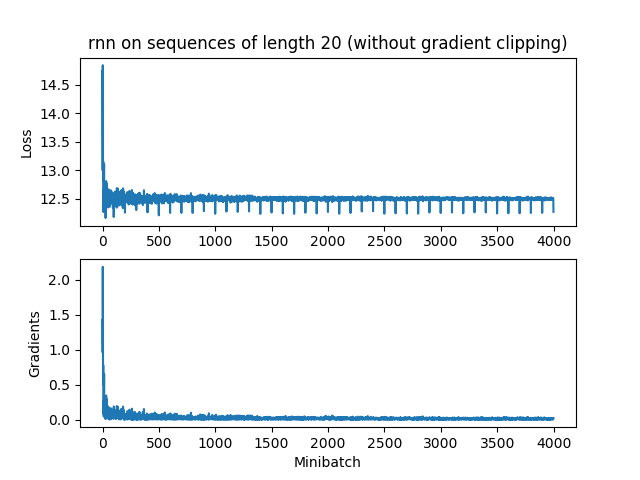
\includegraphics[width=\linewidth]{../assignment3/q3-noclip-rnn.png}
        \caption{rnn no clip}
      \end{center}
    \end{minipage}
    \begin{minipage}{0.5\linewidth}
      \begin{center}
        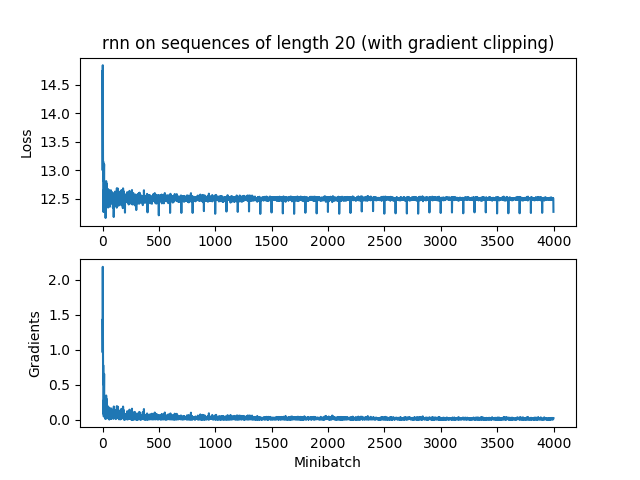
\includegraphics[width=\linewidth]{../assignment3/q3-clip-rnn.png}
        \caption{rnn with clip}
      \end{center}
    \end{minipage}
    \begin{minipage}{0.5\linewidth}
      \begin{center}
        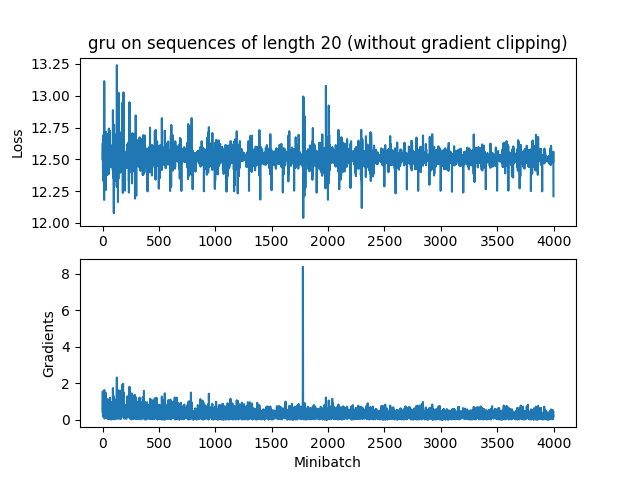
\includegraphics[width=\linewidth]{../assignment3/q3-noclip-gru.png}
        \caption{gru no clip}
      \end{center}
    \end{minipage}
    \begin{minipage}{0.5\linewidth}
      \begin{center}
        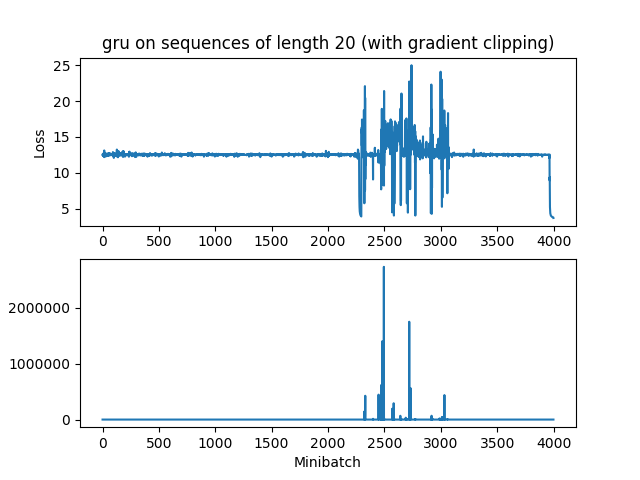
\includegraphics[width=\linewidth]{../assignment3/q3-clip-gru.png}
        \caption{gru with clip}
      \end{center}
    \end{minipage}
  \end{figure}
\end{enumerate}
\end{document}